%%%%%%%%%%%%%%%%%%%%%%%%%%%%%%%%
% SECTION :: IR in our project %
%%%%%%%%%%%%%%%%%%%%%%%%%%%%%%%%
\section{IR in our project}
%%%%%%%%%%%%%%%%%%%%%%%%%%%%%%%%%%%
% Frame Open :: IR in our project %
%%%%%%%%%%%%%%%%%%%%%%%%%%%%%%%%%%%
\frame{\frametitle{IR in our project :: Overflow handled in IR $\rightarrow$ MIPS}
\begin{figure}[htbp]
\begin{center}
% Requires \usepackage{graphicx}
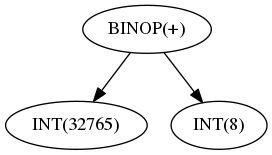
\includegraphics[width=4.0cm]{AST.png}\\
\label{Figure_Simple_Addition_Of_2_Integers_AST}
\end{center}
\end{figure}
\begin{itemize}
\item
Handling arithmetic overflow in the IR $\rightarrow$ MIPS phase
will yield the following (simple) IR code for the addition above:
\begin{itemize}
\item \textbf{li  Temp\_29, 32765}
\item \textbf{li  Temp\_30, 8    }
\item \textbf{add Temp\_31, Temp\_29, Temp\_30}
\end{itemize}
\item
What are the benefits of a simpler IR?
How will the add instruction be translated to MIPS eventually?
\end{itemize}

%%%%%%%%%%%%%%%%%%%%%%%%%%%%%%%%%%%
% Frame Close :: Warm up examples %
%%%%%%%%%%%%%%%%%%%%%%%%%%%%%%%%%%%
}